\chapter{RDBMS}
The relational data model is based on the concept of storing records of data as rows inside tables.
\begin{itemize}
    \item Each \textbf{row} represents an entity of the real world
    \item And each \textbf{column} is an attribute of interest of these entities
\end{itemize}

\section{Relational Data Model}
\subsection{Database and Relation Schemas}
A relational database consists of a set of tables. Each table has
\begin{itemize}
    \item Predefined name: \textbf{relation symbol}
    \item Set of predefined column names \textbf{the attribute names}
    \begin{itemize}
        \item  Each attribute \(A_i\) ranges over a predefined domain \(dom(A_i)\) such that the values in the column can only come from this domain.
    \end{itemize}
\end{itemize}
A table is then filled row-wise like a tuple with values that represent the state of an entity.

The definition of the attribute names \(A_i\) for the relation symbol \(R\) is called a \textbf{relation schema}; the set of the relation schemas of all relation symbols in the database is then called a \textbf{database schema}.

%relational_database_1 AND relational_database_2
\begin{figure}[!hbp]
    \centering
    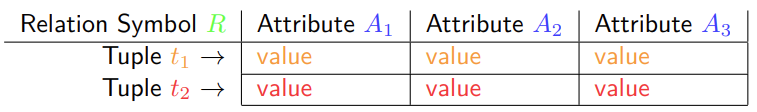
\includegraphics[width=0.90\linewidth]{images/AdvancedDataManagment/rdbms/relational_database_1.png}
    \caption{General example}
\end{figure}
\newpage

\begin{figure}[!hbp]
    \centering
    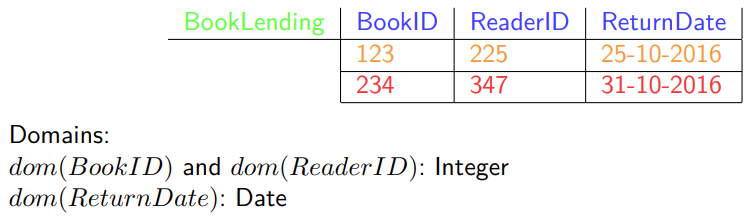
\includegraphics[width=0.90\linewidth]{images/AdvancedDataManagment/rdbms/relational_database_2.png}
    \caption{BookLending example}
\end{figure}

In addition each relation schema can have some type of \textit{constraints} to describe which dependencies between the stored data exist:
\begin{itemize}
    \item \textbf{INTRA relational constraints (local dependencies):} describe dependencies inside a single table, for example be \textit{functional dependencies} – and in particular \textbf{key} constraints
    \item \textbf{INTER relational constraints (global dependencies):} describe dependencies between different tables, for example be \textit{inclusion dependencies} – and in particular \textit{foreign keyindex}
constraints
\end{itemize}

\begin{tcolorbox}
We define a \textbf{Relational Schema} given its
\begin{itemize}
    \item Relation Symbol \(R_i\)
    \item Set of attributes \(A_{i1},...,A_{im}\)
    \item Set of intrarelational/local constraints \(\Sigma_i\)
\end{itemize}
\[R_i = (\{A_{i1},...,A_{im}\}, \Sigma_i)\]
\end{tcolorbox}

\begin{tcolorbox}
We define a \textbf{Database Schema} given its
\begin{itemize}
    \item Database Symbol \(D\)
    \item Set of relation schemas  \(R_1,...,R_m\)
    \item Set of interrelational/global dependencies \(\Sigma\)
\end{itemize}
\[R_i = (\{A_{i1},...,A_{im}\}, \Sigma_i)\]
\end{tcolorbox}

\newpage
\subsubsection{Example Database: Library}
\begin{figure}[!hbp]
    \centering
    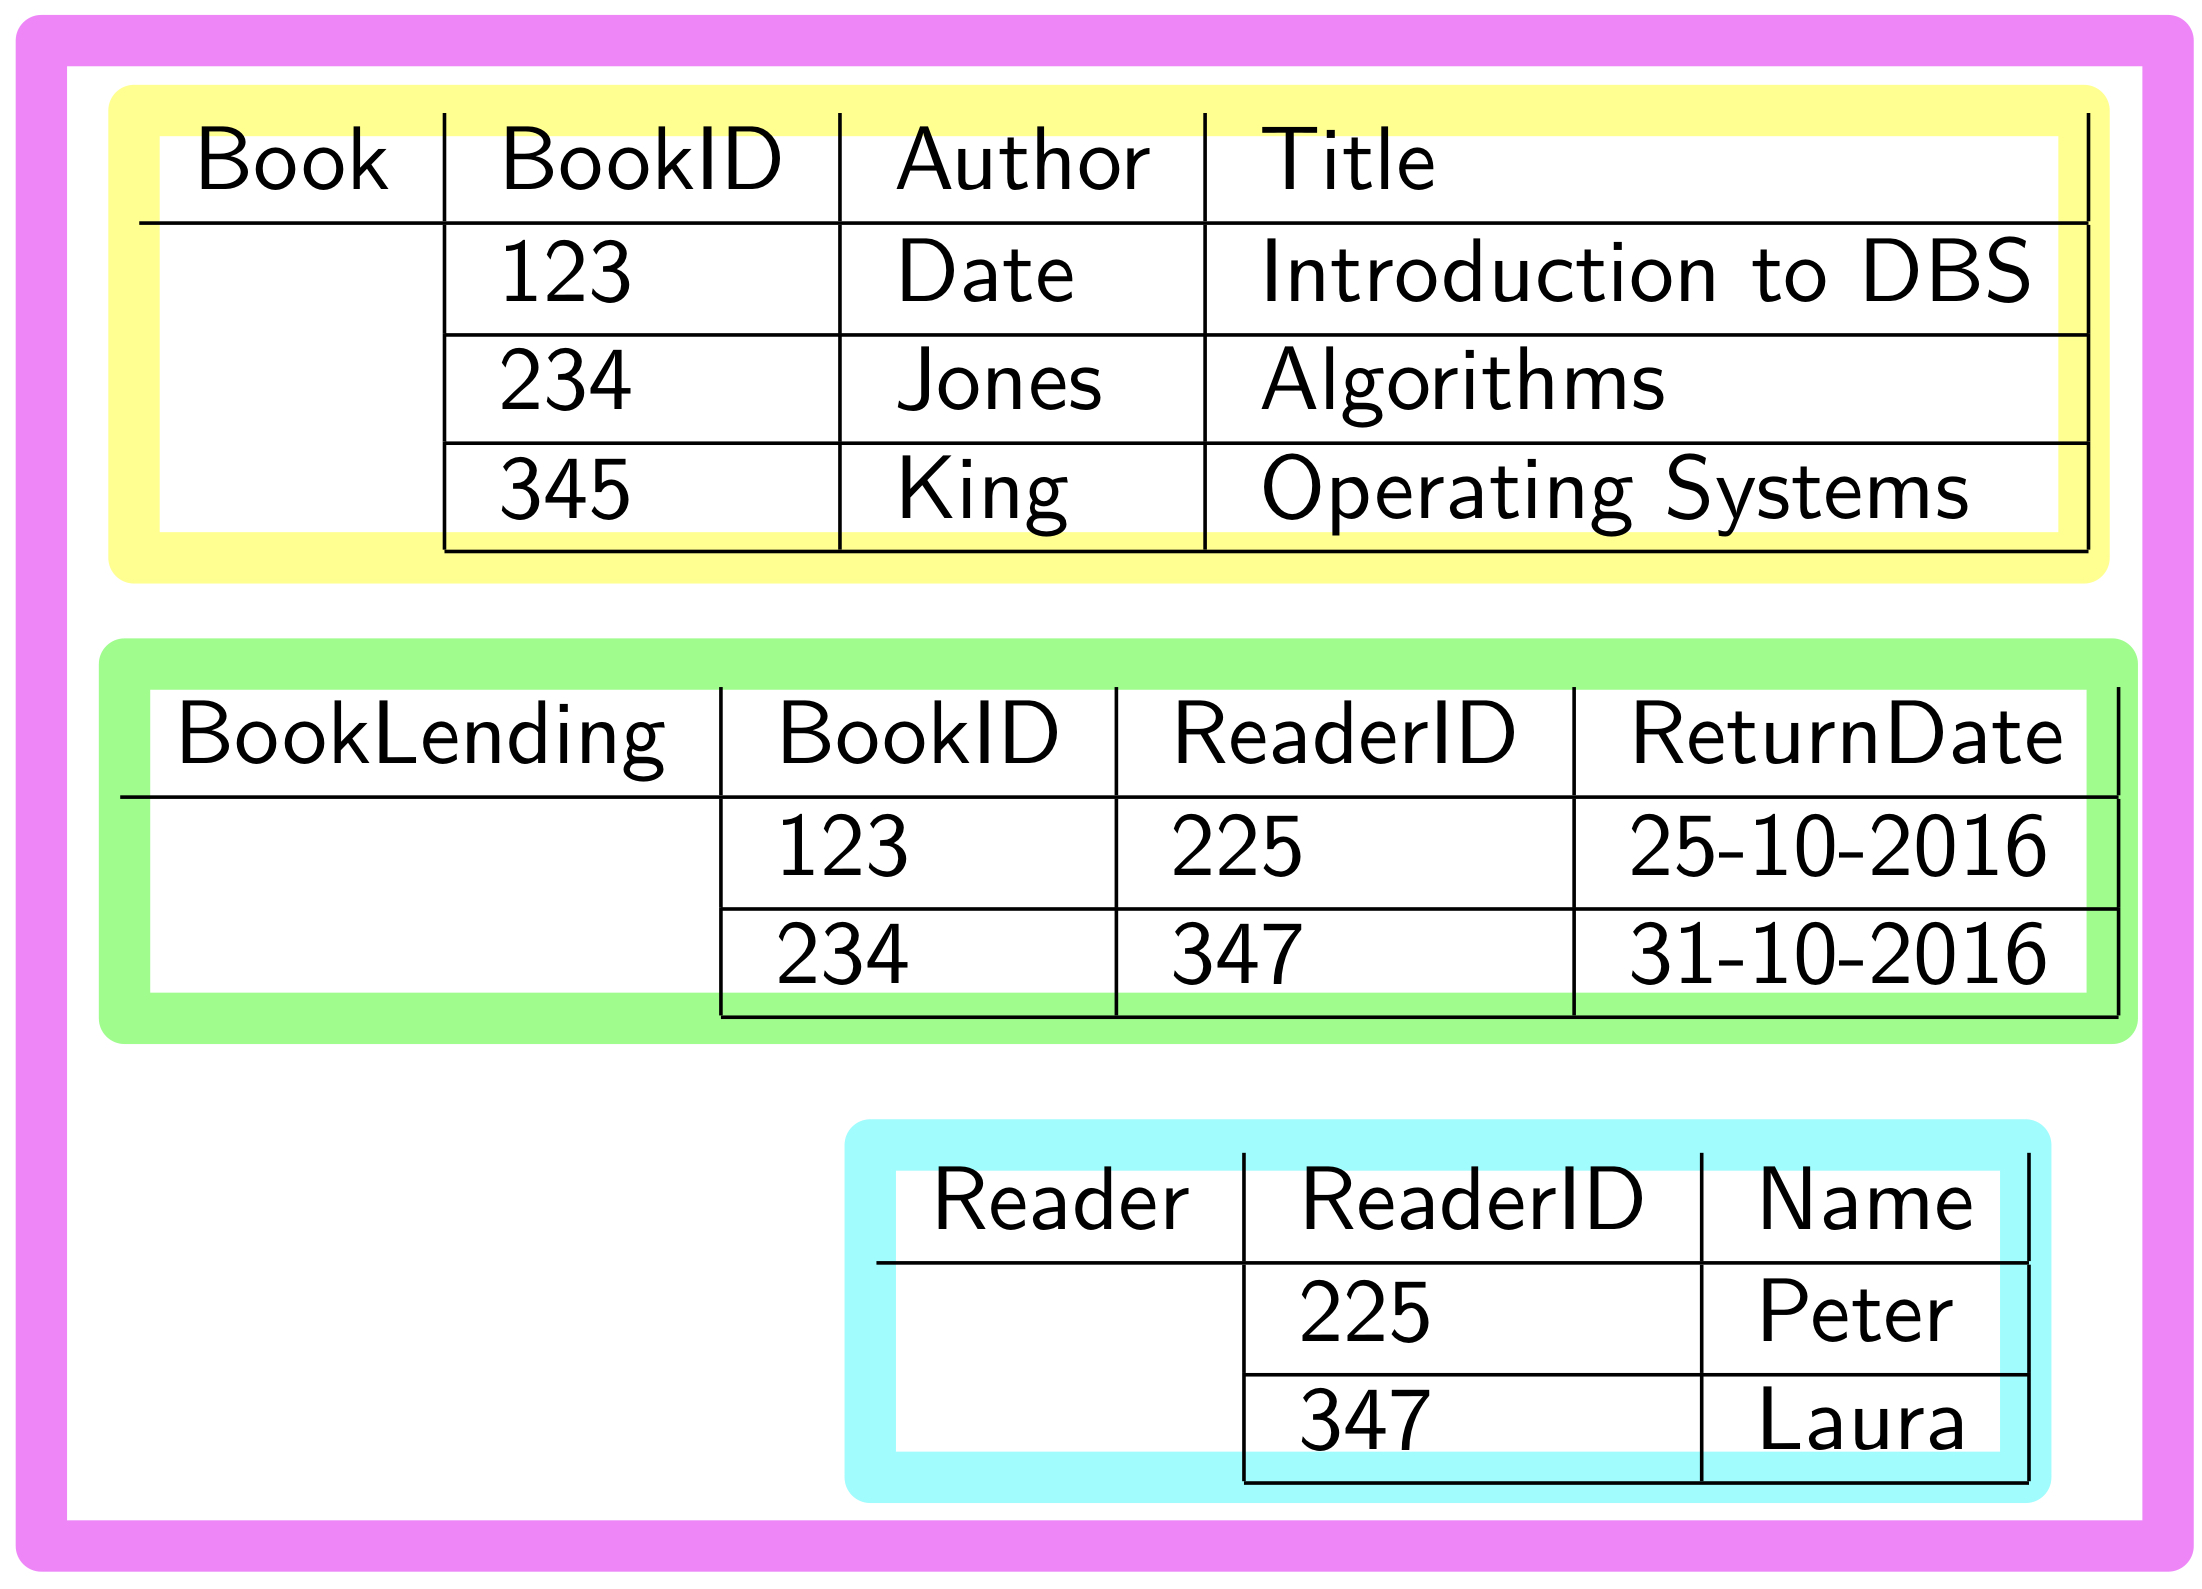
\includegraphics[width=0.60\linewidth]{images/AdvancedDataManagment/rdbms/library_schema_1.jpeg}
    \caption{Library schema example}
\end{figure}

\begin{figure}[!hbp]
    \centering
    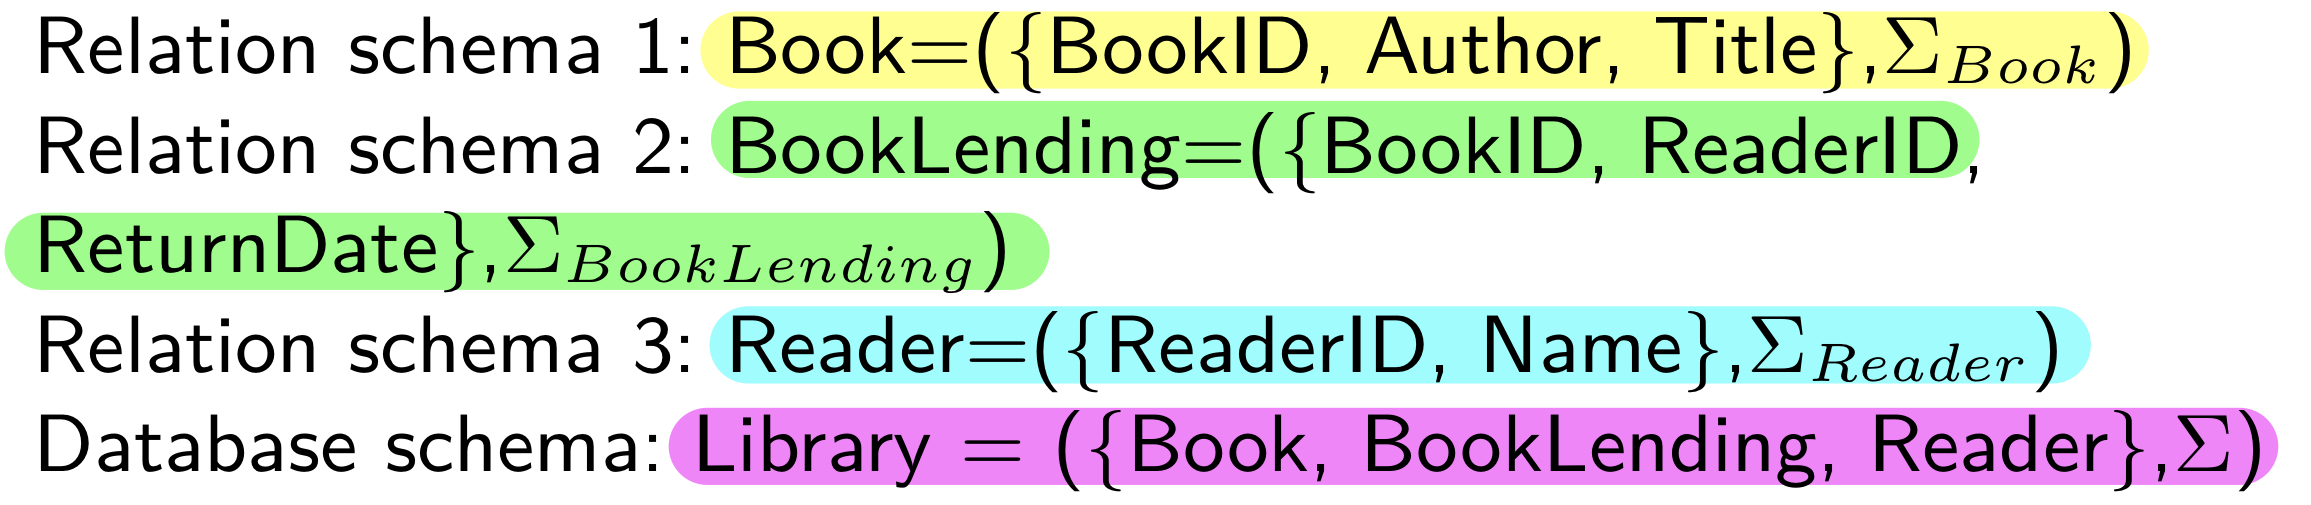
\includegraphics[width=0.70\linewidth]{images/AdvancedDataManagment/rdbms/library_schema2.jpeg}
    \caption{Library schema definition}
\end{figure}

\subsubsection{Example Database: Dependencies}
\begin{figure}[!hbp]
    \centering
    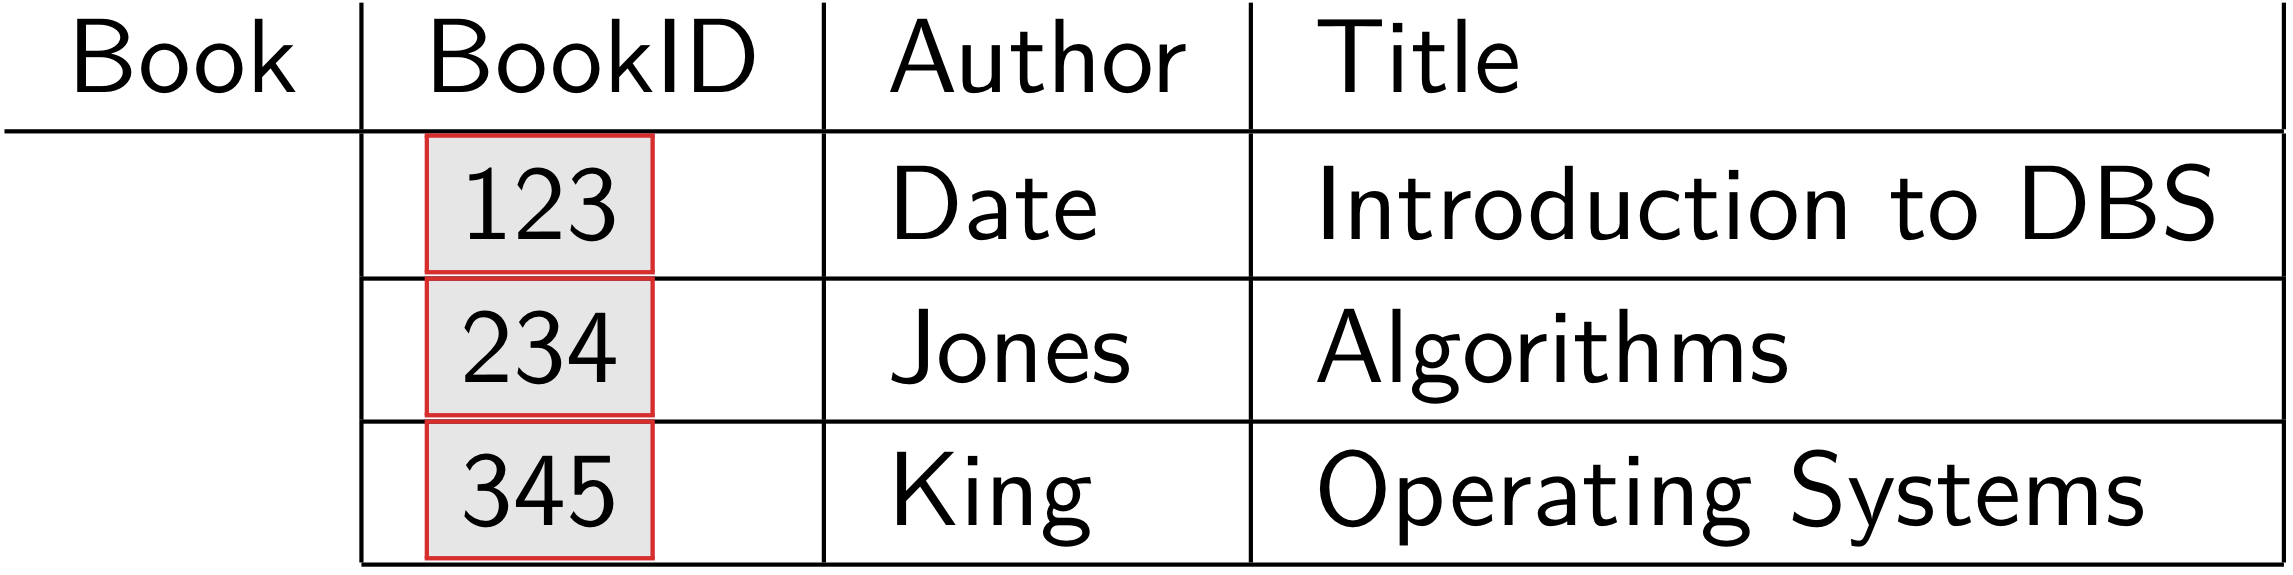
\includegraphics[width=0.50\linewidth]{images/AdvancedDataManagment/rdbms/local_dependencies.jpeg}
    \caption{Book local dependency}
\end{figure}

\begin{figure}[!hbp]
    \centering
    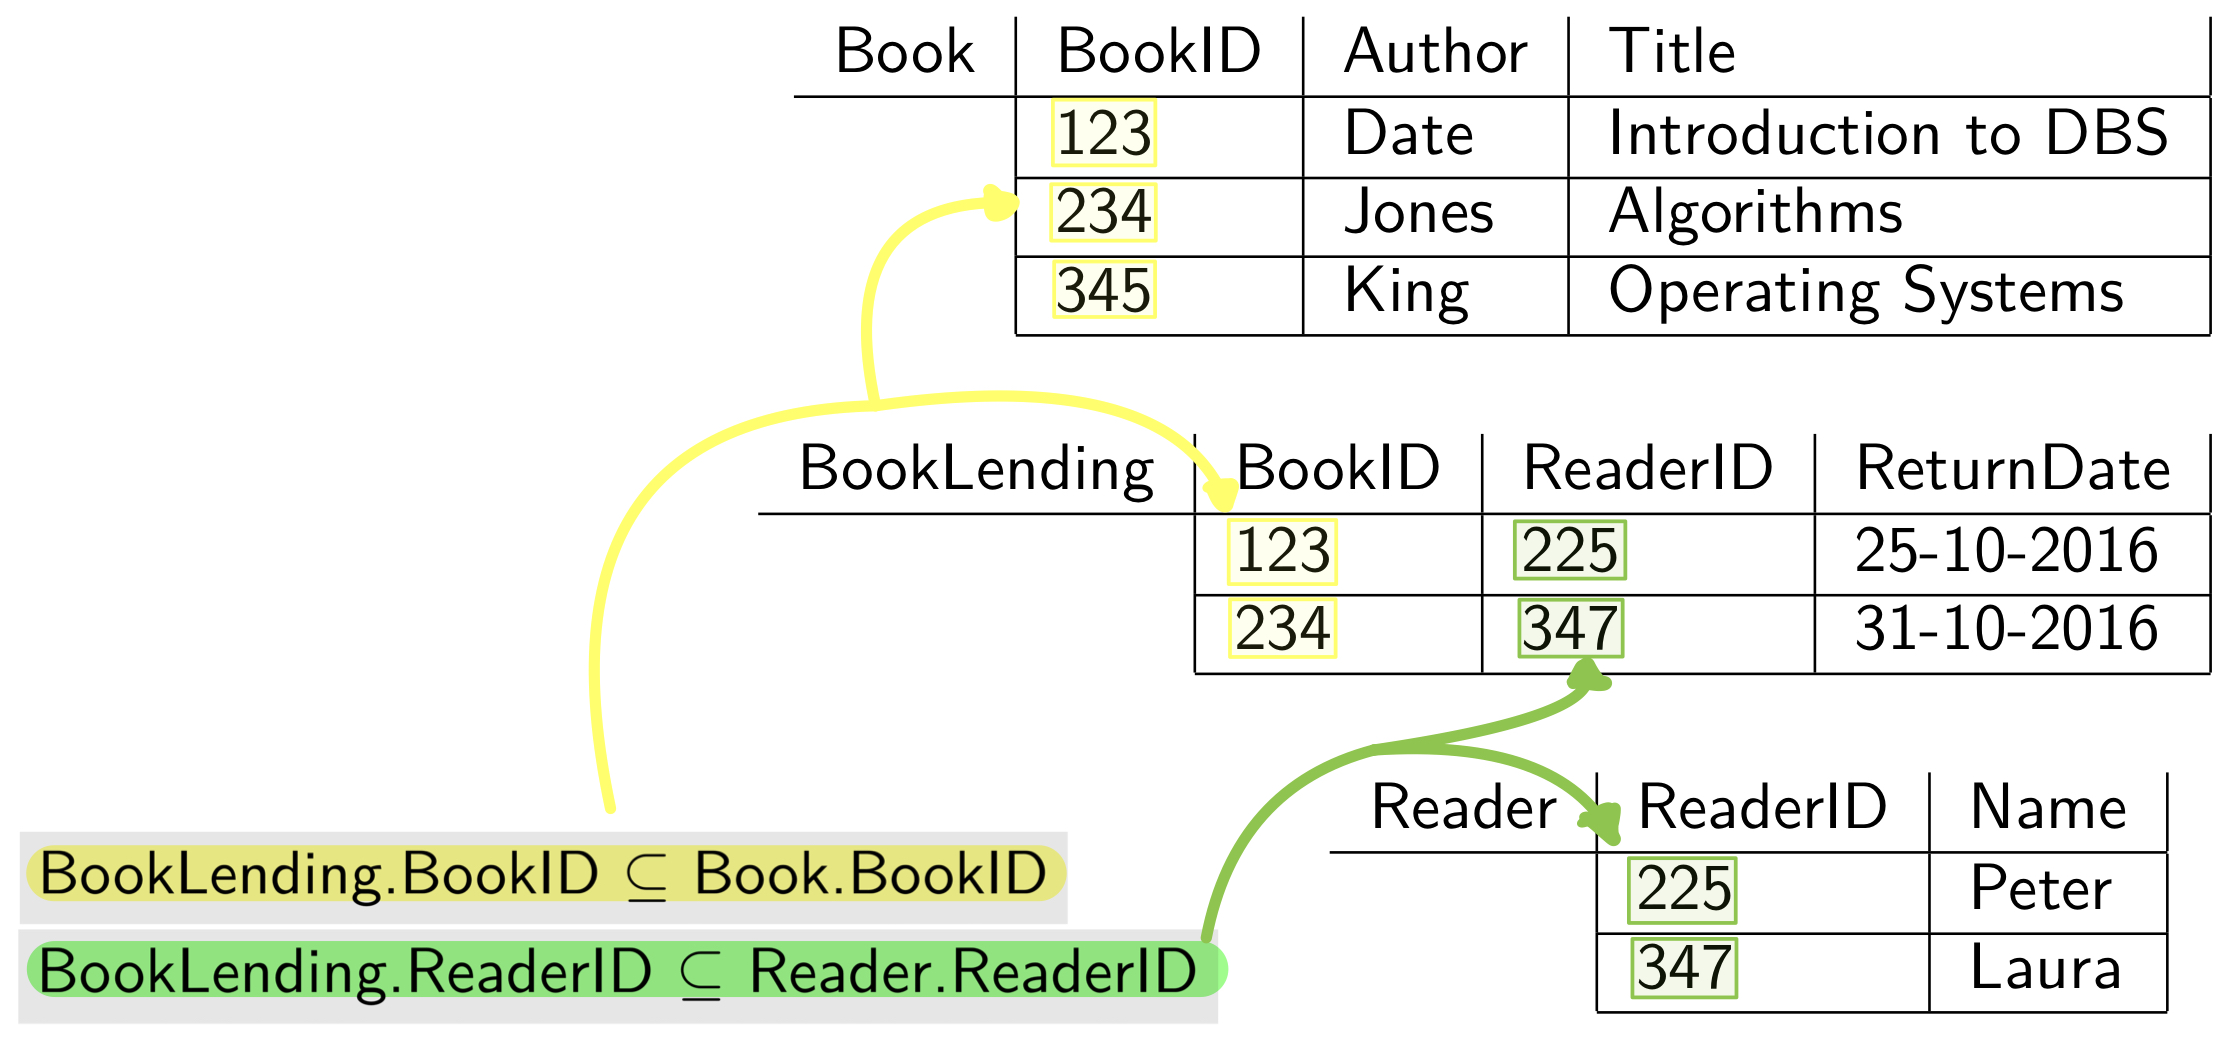
\includegraphics[width=0.70\linewidth]{images/AdvancedDataManagment/rdbms/global_dependencies.jpeg}
    \caption{Library global dependencies}
\end{figure}

\subsection{Mapping ER Models to Schemas}
An ER diagram can be translated into a database schema:
\begin{itemize}
    \item Each \textbf{entity name} corresponds to a relation symbol
    \item Each \textbf{entity attributes} correspond to relation attributes
    \begin{itemize}
        \item Relational data model does not allow multi-valued ad composite attributes
        \item In the case of multi-valued attributes, a new relation schema for each multi-valued attribute created containing additional foreign keys 
    \end{itemize}
    \item \textbf{Composite attributes} should usually be treated as single-valued attributes
    \item \textbf{Relationship} are also translated into a relation schema. In order to be able to map the values from the entities connected by the relationship together, the relation also contains the key attributes of the entities participating in the relationship
\end{itemize}

\subsection{Normalization}
Some database designs are problematic, they contain too many attributes, or tables combine the “wrong” attributes, or tables store data duplicates. These problem cause problem when \textit{inserting}, \textit{deleting} or \textit{updating values}: they are called \textbf{anomalies}, and there are many types like:
\begin{itemize}
    \item \textbf{Insertion anomaly:} we need all attribute values before inserting a tuple
    \item \textbf{Deletion anomaly:} when deleting a tuple, information is lost that we still need in the database
    \item \textbf{Update anomaly:} when data are stored redundantly, values have to be changed in more than one tuple
\end{itemize}
\begin{tcolorbox}
Normalization results in a good distribution of the attributes among the tables and hence normalization helps reduce anomalies. Moreover it depends on the functional dependencies of the relative data table.
\end{tcolorbox}

We have seen 3 main types of Normal form:
\begin{enumerate}
    \item \textbf{First Normal Form (1NF)} that erase the multi-valued and allow composite attributes
    \item \textbf{Second Normal Form (2NF)} in which all non-key attributes are fully dependent on the key attributes
    \item \textbf{Third Normal From (3NF)} in which all non-key attributes are directly dependent on the key attributes
\end{enumerate}

\newpage
\subsubsection{Example of Normalization}
\begin{figure}[!hbp]
    \centering
    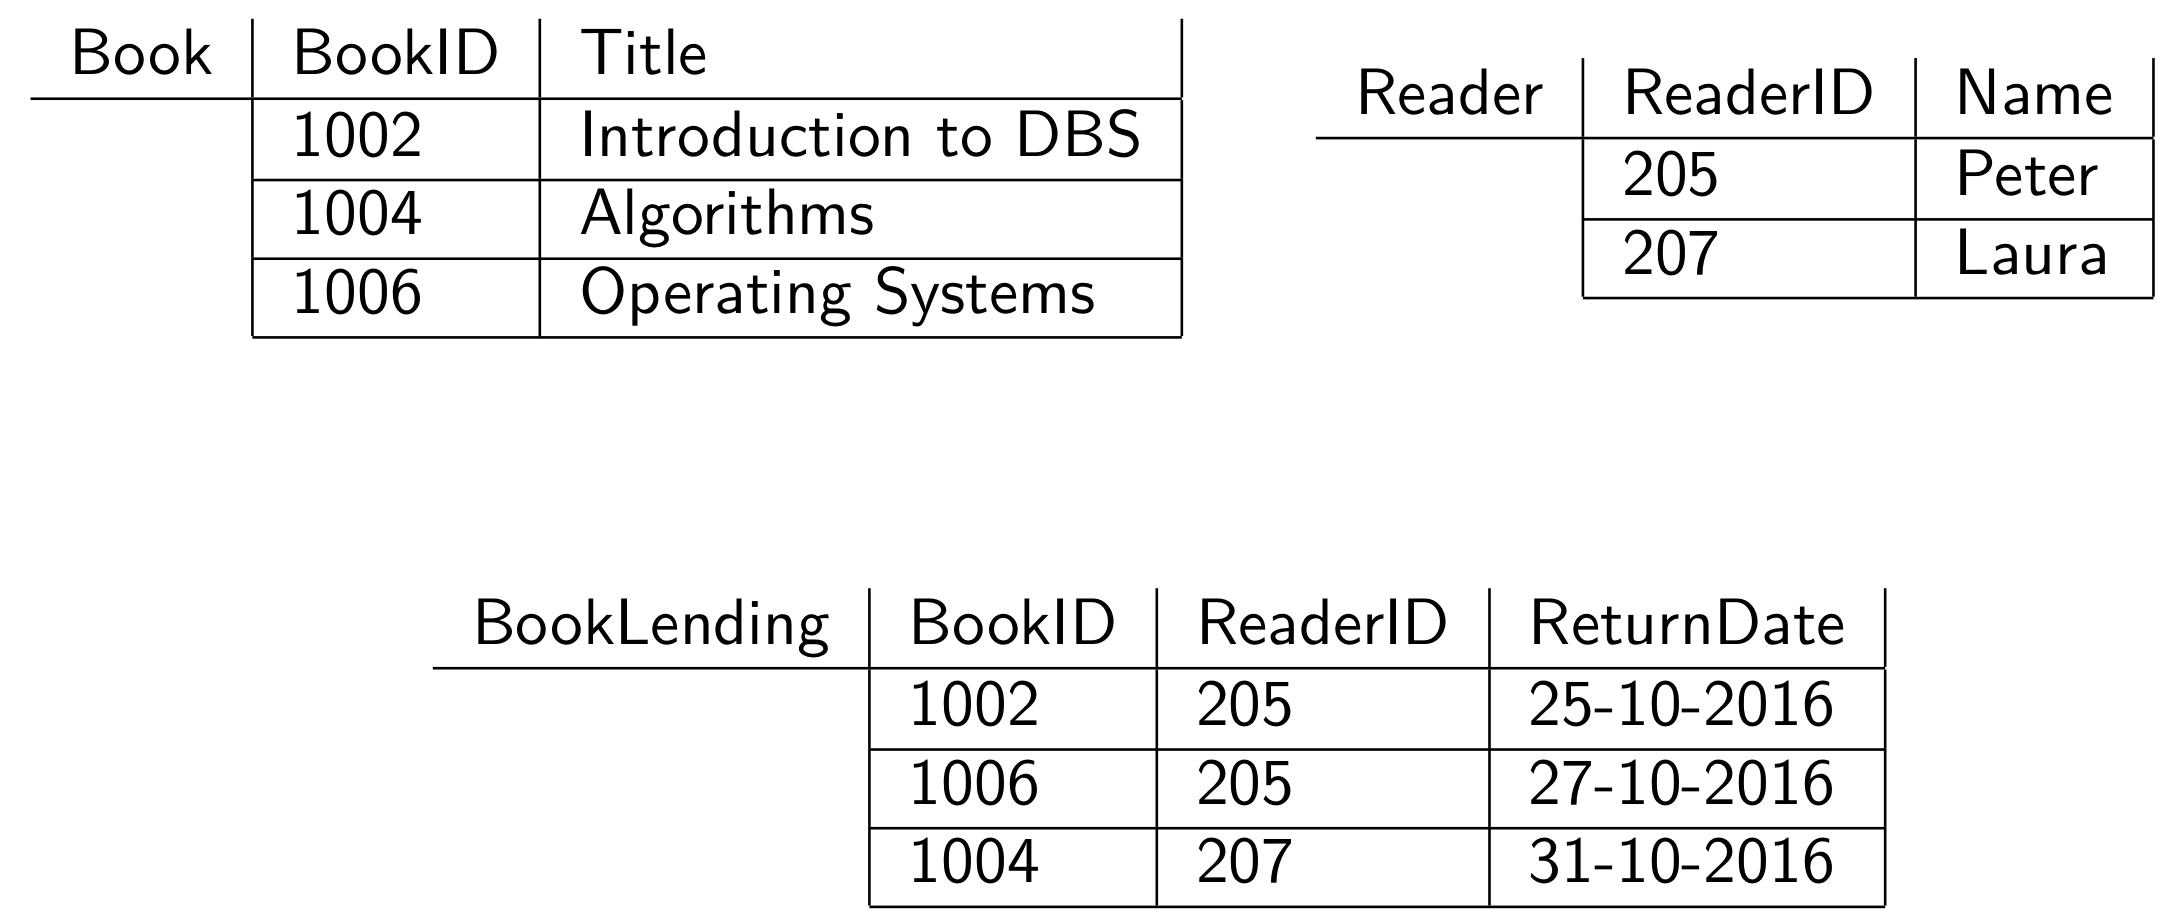
\includegraphics[width=0.70\linewidth]{images/AdvancedDataManagment/rdbms/normalization.jpeg}
    \caption{Library schema normalized}
\end{figure}

\section{Relational Query Languages}
After having design the relational database the next point is to define a strategy to retrieve some information, update and insert additional data in our just born database. We can choose on different strategy, for example taking into account the previous Library example, there is:
\begin{itemize}
    \item \textbf{Natural Language:} "Find all lent books that must be returned before 29-10-2016"
    \item \textbf{Relational Calculus:} Logical formula with variables \(x, y, z:\)
    \[Q(x,y,z) = \{(x,y,z)|\text{BookLending}(x,y,z)\ \land z < \text{29-10-2016}\}\]
    \item \textbf{Relational Algebra} \(\sigma_{ReturnDate<29-10-2016}(BookLending)\)
\end{itemize}

\subsection{Relational Algebra Operators}
\begin{itemize}
    \item \textbf{Projection \(\pi\)} to make some attribute restriction. IDs of readers currently reading a book: \(\pi_{ReaderID}(BookLending)\)
    \item \textbf{Selection \(\sigma\)} with condition on answer tuples. All books to be returned before 29-10-2016: \(\sigma_{ReturnDate<29-10-2016}(BookLending)\)
    \item \textbf{Renaming \(\rho\)} to assign a new attribute name. Rename ReturnDate to DueDate \(\rho_{DueDate\leftarrow ReturnDate}(BookLending)\)
    \item \textbf{Union, Difference and Intersection}
    \item \textbf{Natural Join \(\Join\)} to combine two tables on attributes with same name. All information on Books currently lent: \(\text{Book} \Join \text{BookLending}\)
\end{itemize}
One more thing to note about relational algebra is that an algebra query can be illustrated by a tree:
\begin{itemize}
    \item \textit{Inner nodes} are the algebra operators
    \item \textit{Leaf nodes} are the relation symbol
\end{itemize}

\section{Transaction}
A transaction can be characterized as a sequence of read and write operations on a database; this sequence of operations must be treated as a whole and cannot be interrupted. A transaction moves our system state from one into an other. The following propriety are ensured:
\begin{itemize}
    \item \textbf{Logical data integrity:} are the written values correct and final results of a computation?
    \item \textbf{Physical data integrity \& Recovery:} how can correct values be restored after a system crash?
    \item \textbf{Multi-user support:} how can users concurrently operate on the same database without interfering?
\end{itemize}
To achieve physical data integrity and as part of the recovery management, the database system maintains a \textbf{transaction log}. It stores which operation of which transaction is currently being executed. After a system restart all operations of uncommitted transactions have to be undone. The transaction log also has to take care of committed transactions: If all results of a transaction have been computed but disk writing is interrupted, after a system restart all affected computations of the transaction have to be redone and then stored to disk.


Most RDBMS manage transactions according to the following properties:
\begin{itemize}
    \item \textbf{A}tomicity: either execute all operations or none of them
    \item \textbf{C}onsistency: after the transaction, all values in the database are correct
    \item \textbf{I}solation: concurrent transactions of different users do not interfere
    \item \textbf{D}urability: all transaction results persist in the database even after a system crash
\end{itemize}
